% !TEX root = ../YourName-Dissertation.tex

\chapter{Direct Measurement of the Neutrino Mass with Cyclotron Radiation Emission Spectroscopy}

\section{Introduction}

\section{Cyclotron Radiation Emission Spectroscopy}

\begin{figure}[htbp]
    \centering
    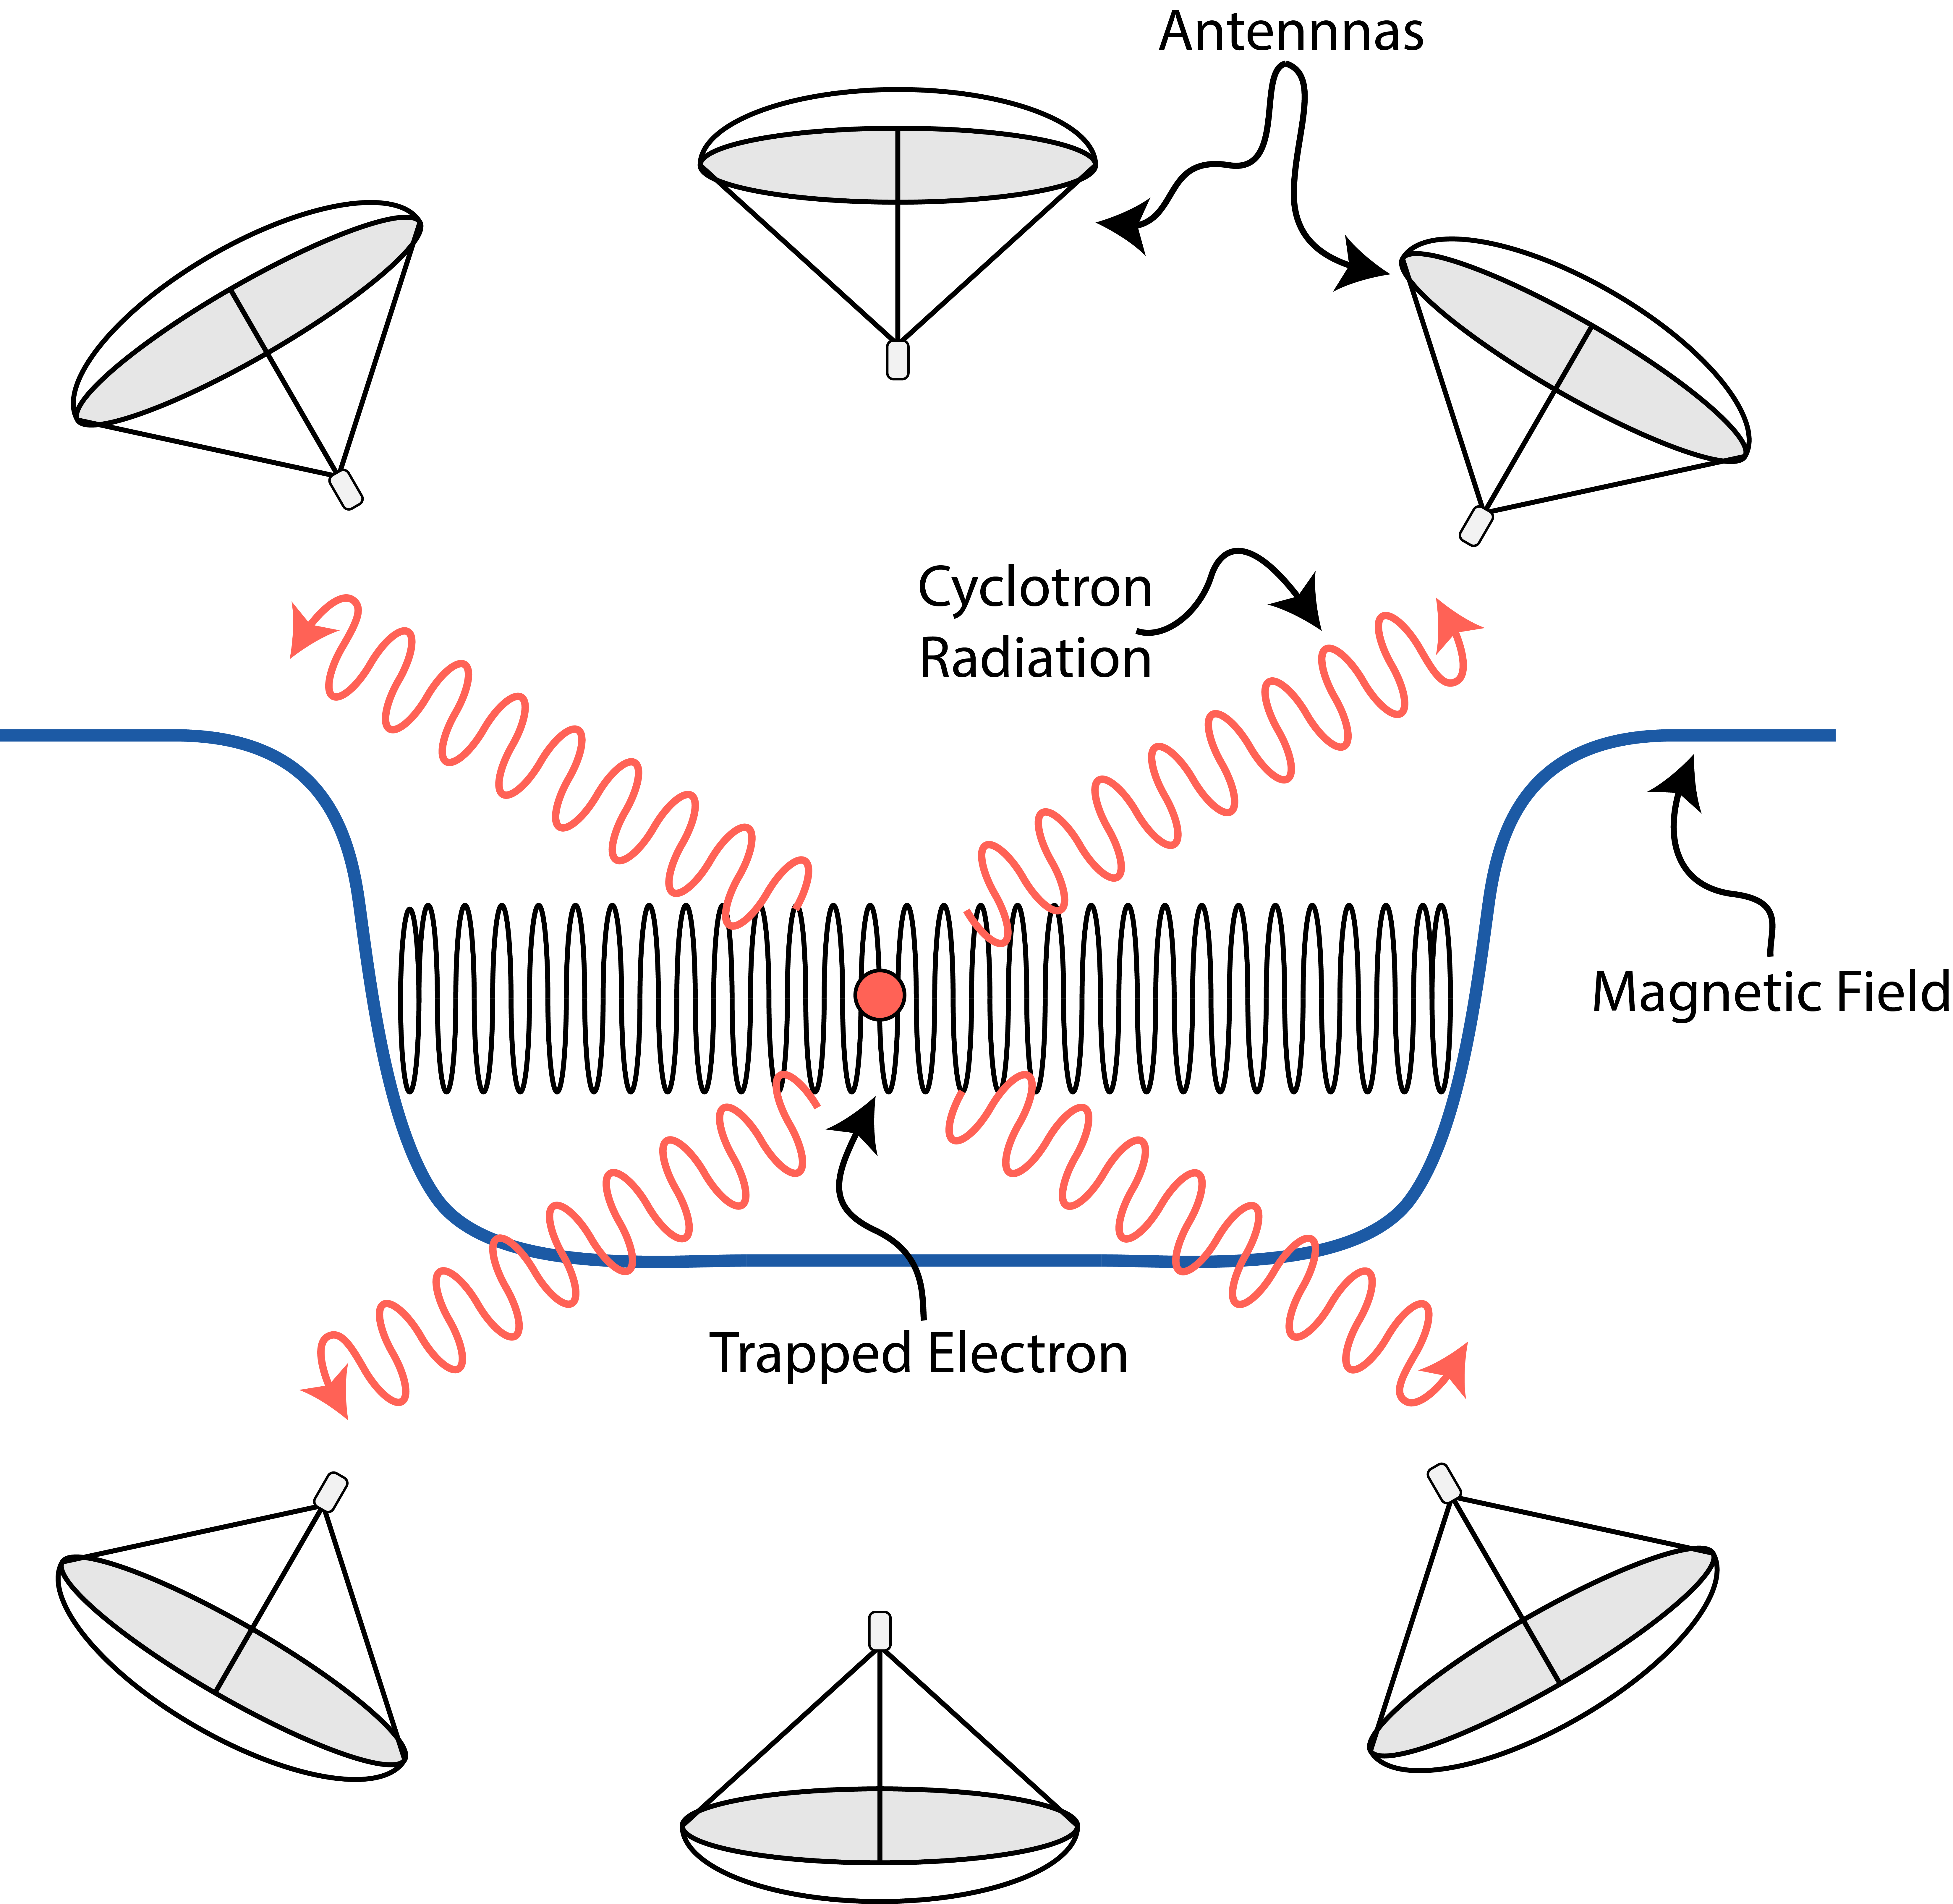
\includegraphics[width=0.5\textwidth]{figs/Chapter-3/230303_cres_cartoon.png}
    \caption{Caption}
    \label{fig:cres_cartoon}
\end{figure}

\subsection{Charged Particles in a Magnetic Trap}

\begin{figure}[htbp]
    \centering
    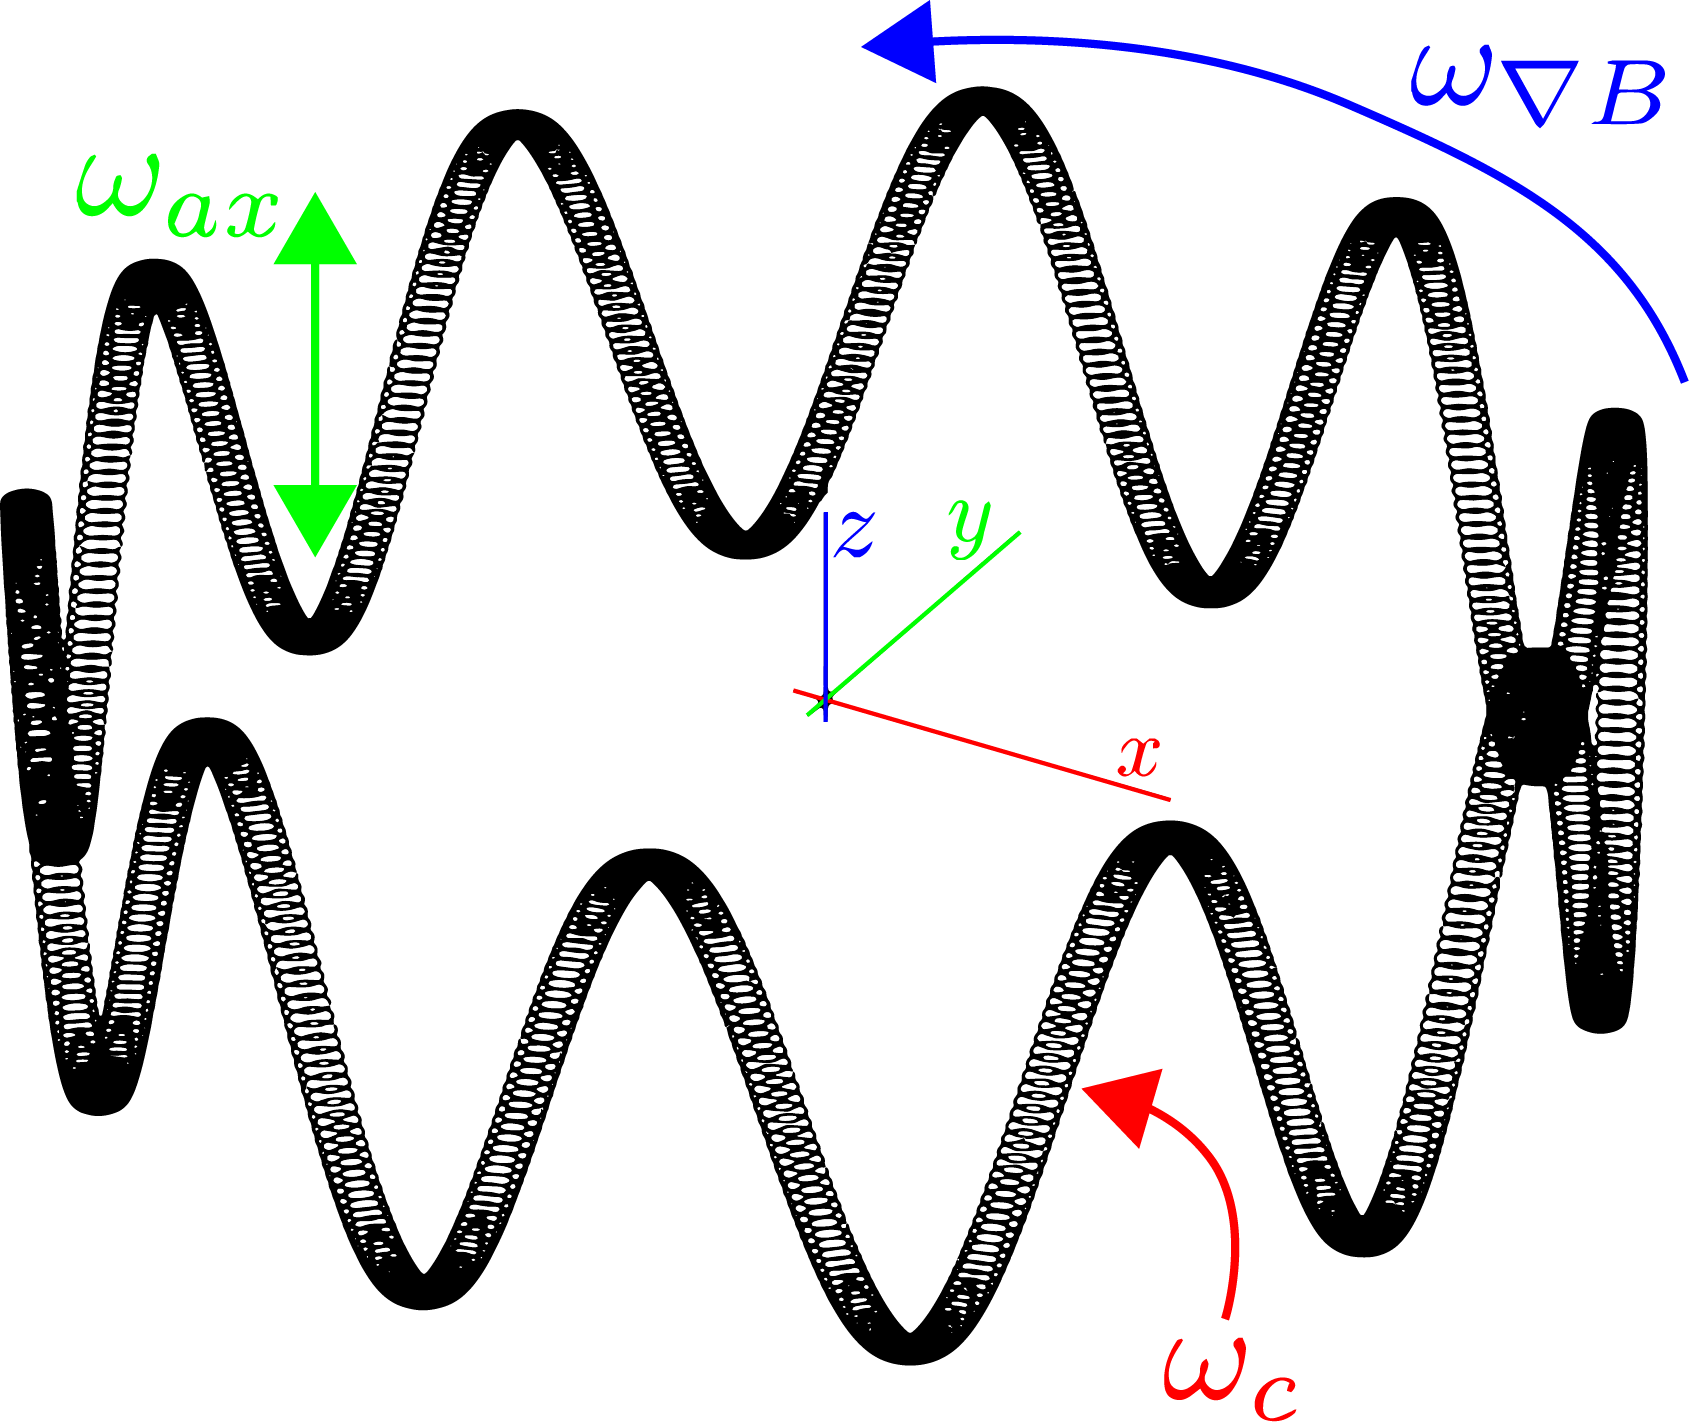
\includegraphics[width=0.5\textwidth]{figs/Chapter-3/230511_trapped_motion.png}
    \caption{Caption}
    \label{fig:chap3-trapped-electron-motion}
\end{figure}

\subsection{Radiation from a Charged Particle}

\section{The Project 8 Collaboration}

\begin{figure}[htbp]
    \centering
    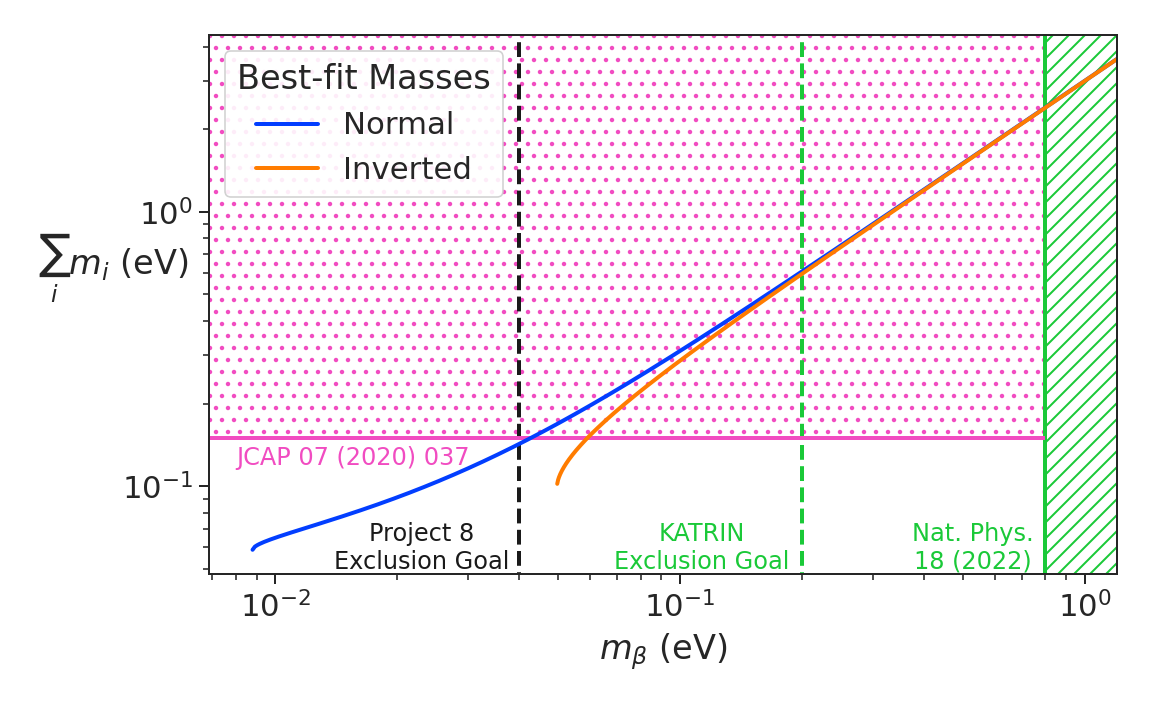
\includegraphics[width=0.7\textwidth]{figs/Chapter-3/230303_sum_nu_mass_vs_m_beta_with_exclusion_and_goal.png}
    \caption{Caption}
    \label{fig:p8_nu_mass_goal}
\end{figure}

\section{First Tritium Beta Decay Spectrum and Neutrino Mass Measurment with CRES}

\subsection{The Project 8 CRES Demonstrator}

\begin{figure}[htbp]
    \centering
    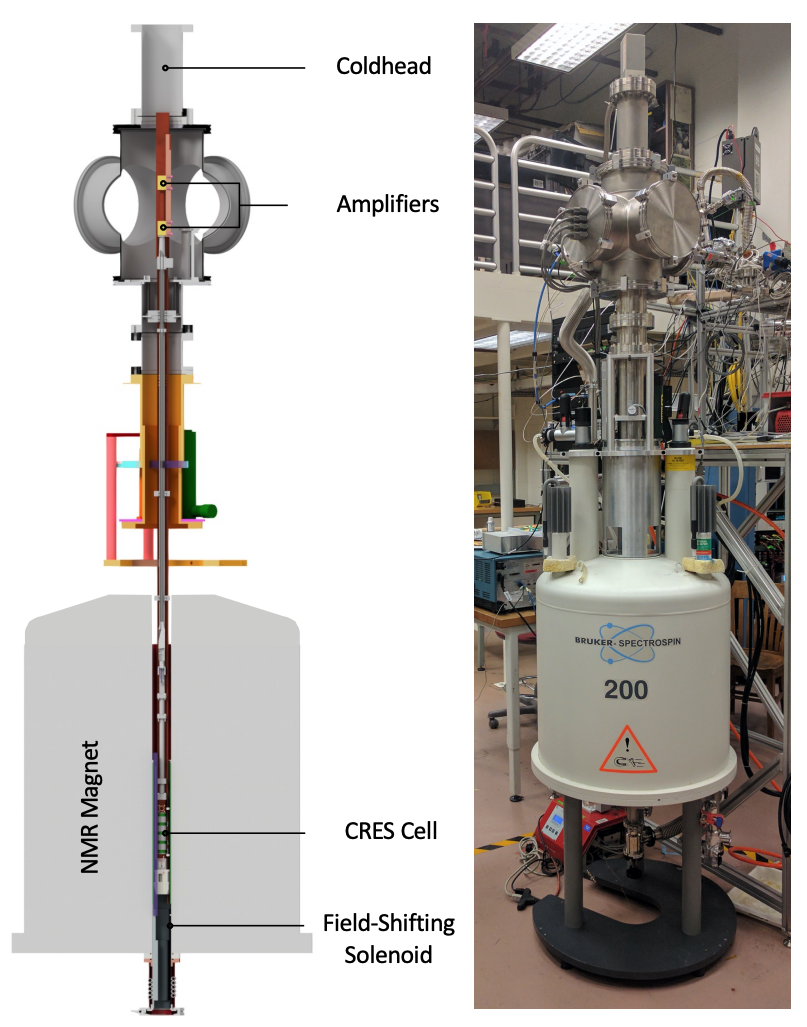
\includegraphics[width=0.7\textwidth]{figs/Chapter-3/phaseII_system.png}
    \caption{Caption}
    \label{fig:phase2_apparatus}
\end{figure}

\begin{figure}[htbp]
    \centering
    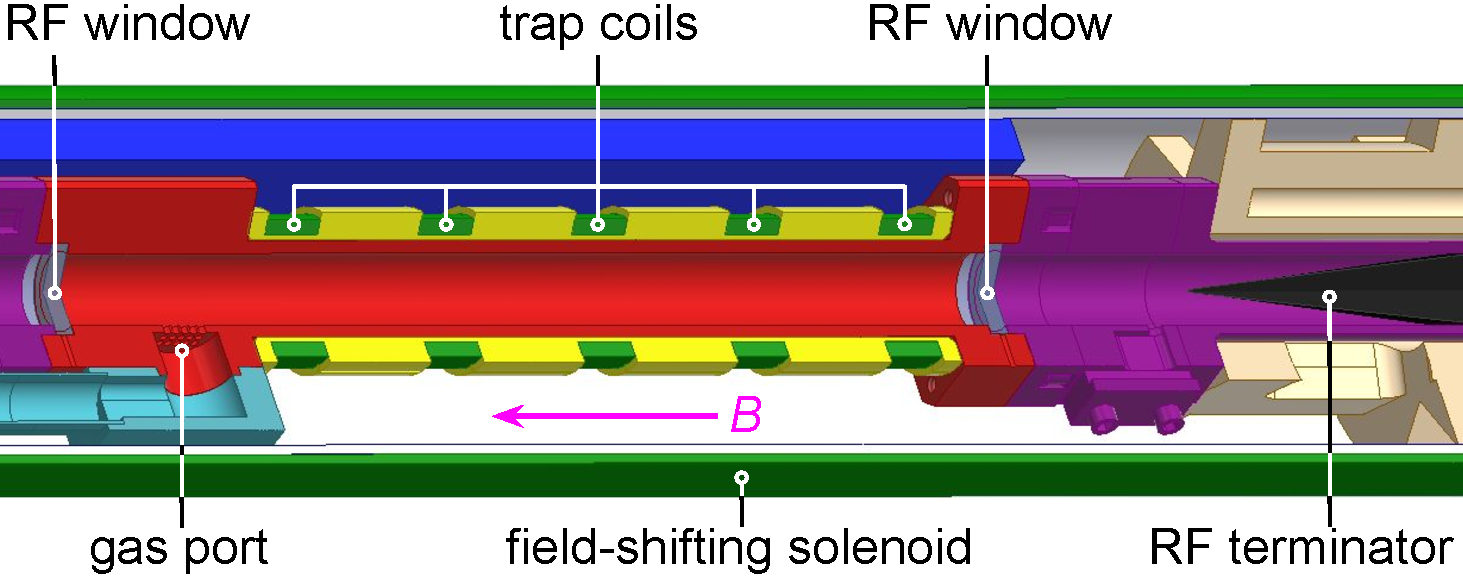
\includegraphics[width=0.8\textwidth]{figs/Chapter-3/apparatus.pdf}
    \caption{Caption}
    \label{fig:phase2_cres_cell}
\end{figure}

\subsection{CRES Track and Event Reconstruction}

\begin{figure}[htbp]
    \centering
    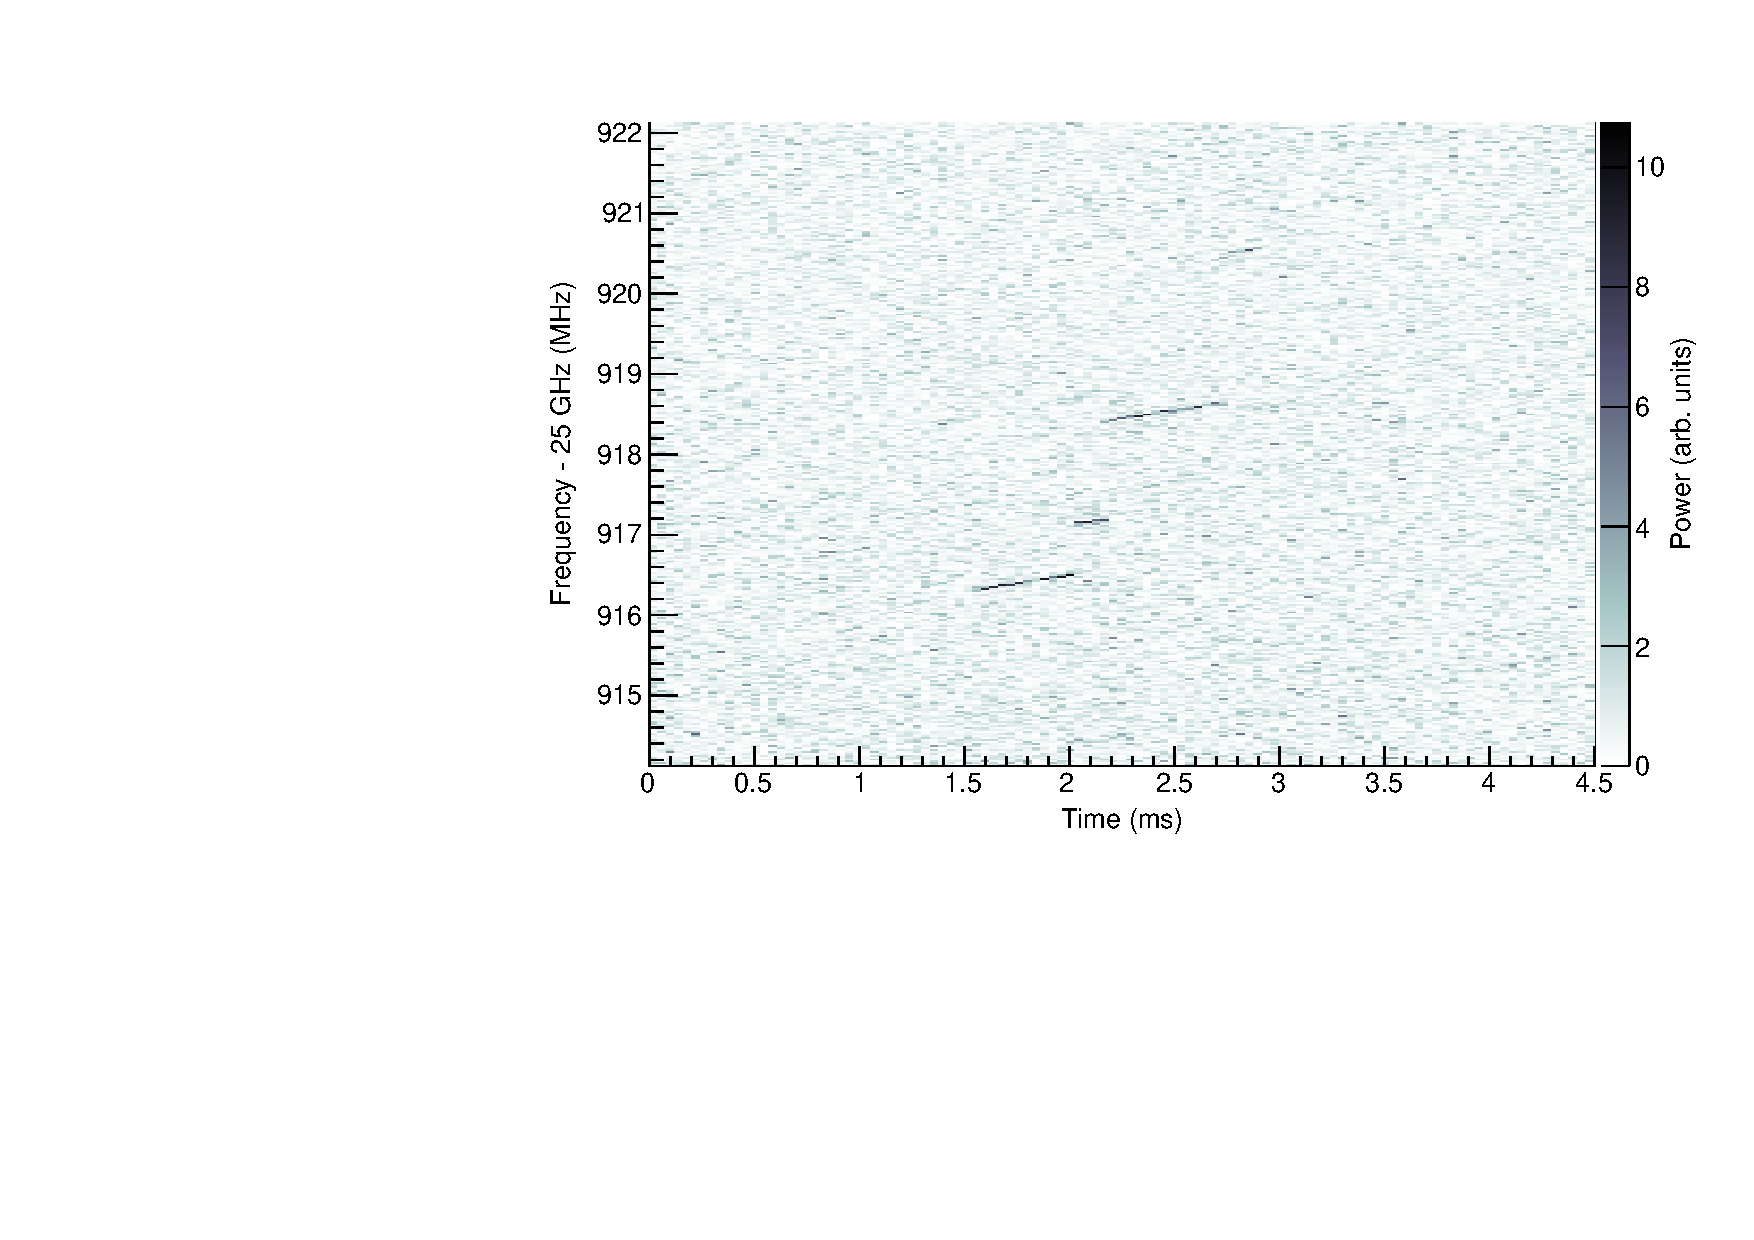
\includegraphics[width=0.7\textwidth]{figs/Chapter-3/T2_Event0.pdf}
    \caption{Caption}
    \label{fig:tritium_event0}
\end{figure}

\subsection{Measurements with Krypton}

\begin{figure}[htbp]
    \centering
    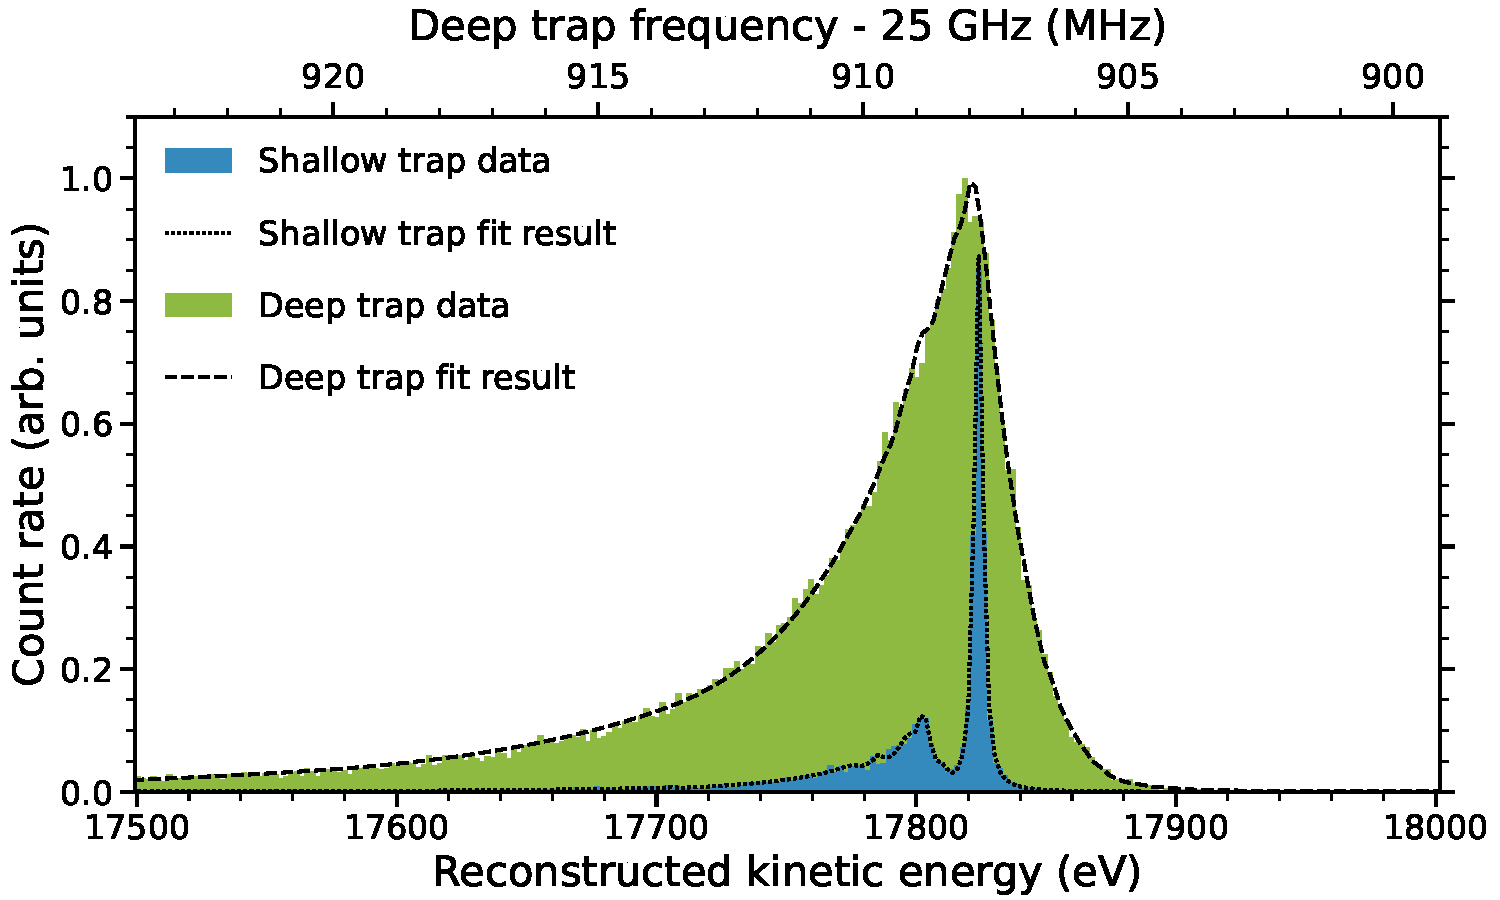
\includegraphics[width=0.7\textwidth]{figs/Chapter-3/kr_fit.pdf}
    \caption{Caption}
    \label{fig:krypton_fit}
\end{figure}

\begin{figure}[htbp]
    \centering
    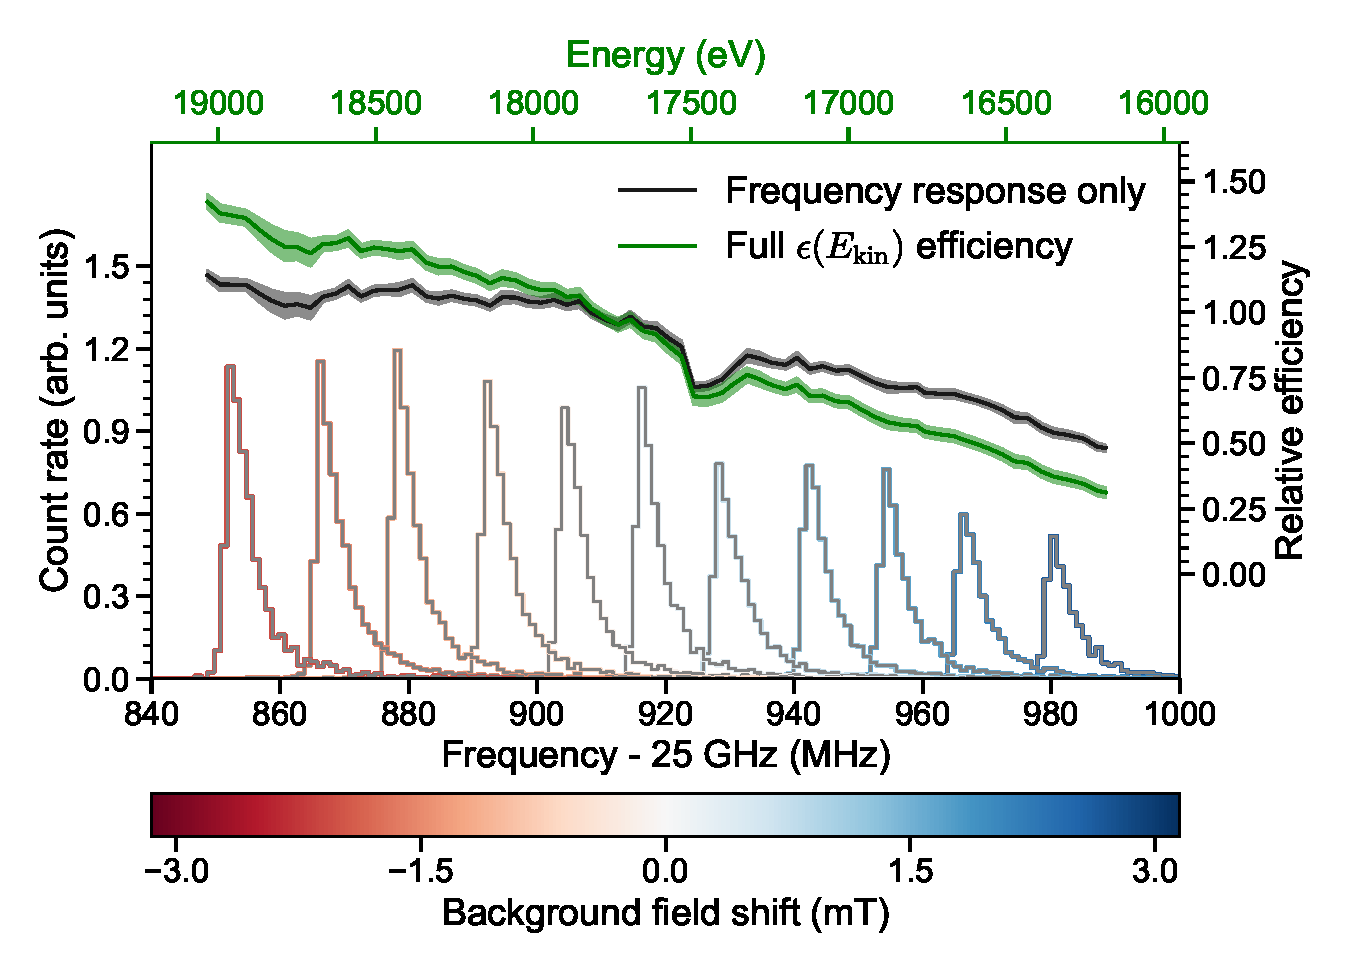
\includegraphics[width=0.7\textwidth]{figs/Chapter-3/fss_for_prl_plot.pdf}
    \caption{Caption}
    \label{fig:fss_plot}
\end{figure}

\subsection{Tritium Spectrum and Neutrino Mass Results}

\begin{figure}
    \centering
    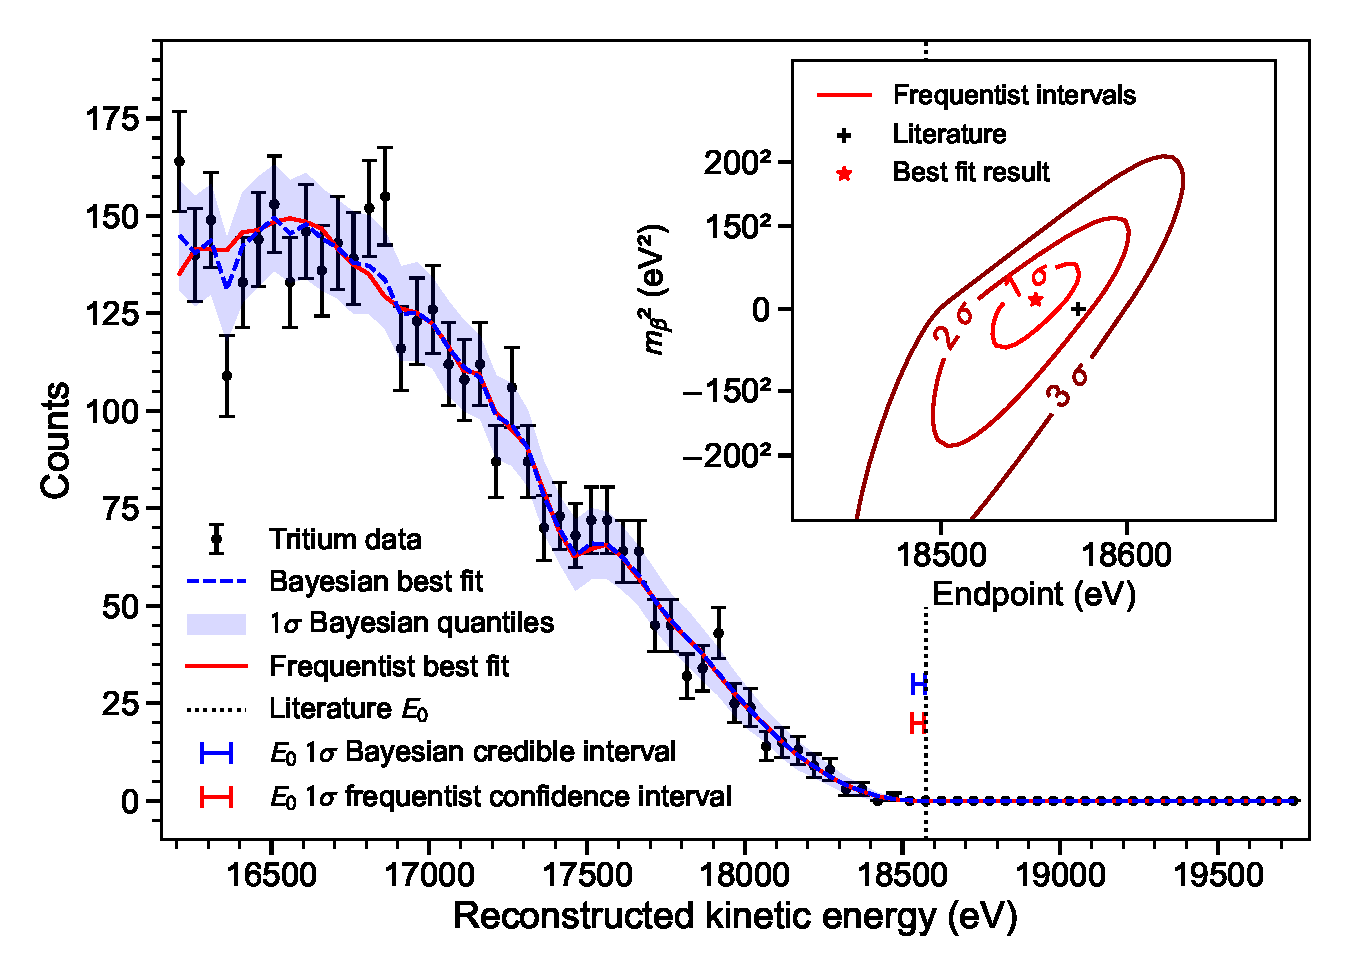
\includegraphics[width=0.7\textwidth]{figs/Chapter-3/12-03-22A_final_E0_real_data_phase_II_tritium_fit_1d.pdf}
    \caption{Caption}
    \label{fig:final_tritium_fit}
\end{figure}

\section{Scalable Approaches to CRES Measurements}
\subsection{The Antenna Array Approach}
\subsection{The Cavity Approach}



